% !TeX spellcheck = cs_CZ
%{\tikzset{external/prefix={tikz/FYZII/}}
% \tikzset{external/figure name/.add={ch37_}{}}
%---------------------------------------------------------------------------------------------------
% file fey2ch37.tex
%---------------------------------------------------------------------------------------------------
%=========================== Kapitola Magnetické látky =============================================
\setchaptertoc
\chapter{Magnetické látky}\label{fyz:IIchapXXXVII}

  \section{Podstata feromagnetizmu}\label{fyz:IIchapXXXVIIsecI}
  \section{Termodynamické vlastnosti}\label{fyz:IIchapXXXVIIsecII}
  \section{Hysterezní smyčka}\label{fyz:IIchapXXXVIIsecIII}
  \section{Feromagnetické látky}\label{fyz:IIchapXXXVIIsecIV}
  \section{Zvláštní magnetické látky}\label{fyz:IIchapXXXVIIsecV}

    \begin{figure}[ht!] %\ref{fyz:fig0817}
      \centering
      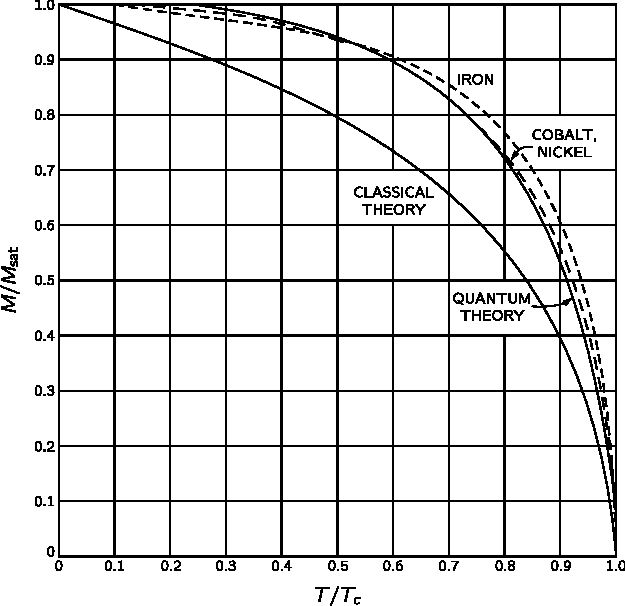
\includegraphics[width=0.7\linewidth]{fyz_fig0817.pdf}
      \caption{
               (\cite[s.~707]{Feynman02})}
      \label{fyz:fig0817}
    \end{figure}

    \begin{figure}[ht!]
      \centering
      \subcaptionbox{\label{fyz:fig0818a}}{\luafigure[0.9]{fyz_fig0818a.pdf}}               \\
      \subcaptionbox{\label{fyz:fig0818b}}{\luafigure[0.9]{fyz_fig0818b.pdf}}               \\
      \subcaptionbox{\label{fyz:fig0818c}}{\luafigure[0.9]{fyz_fig0818c.pdf}}
      \caption{
               (\cite[s.~748]{Feynman02})}
      \label{fyz:fig0818}
    \end{figure}

    \begin{figure}[ht!] %\ref{fyz:fig0819}
      \centering
      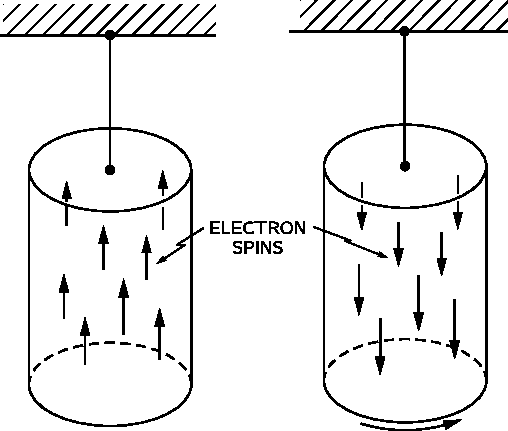
\includegraphics[width=0.7\linewidth]{fyz_fig0819.pdf}
      \caption{
               (\cite[s.~707]{Feynman02})}
      \label{fyz:fig0819}
    \end{figure}

    \begin{figure}[ht!] %\ref{fyz:fig0820}
      \centering
      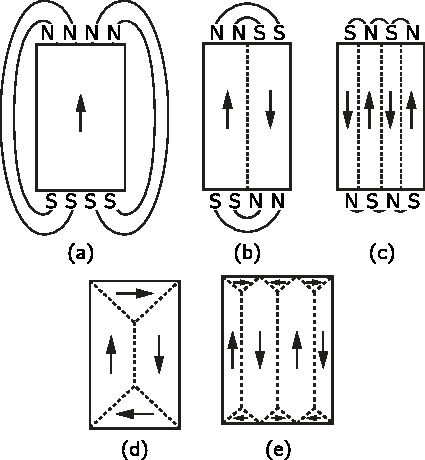
\includegraphics[width=0.7\linewidth]{fyz_fig0820.pdf}
      \caption{
               (\cite[s.~707]{Feynman02})}
      \label{fyz:fig0820}
    \end{figure}

    \begin{figure}[ht!] %\ref{fyz:fig0821}
      \centering
      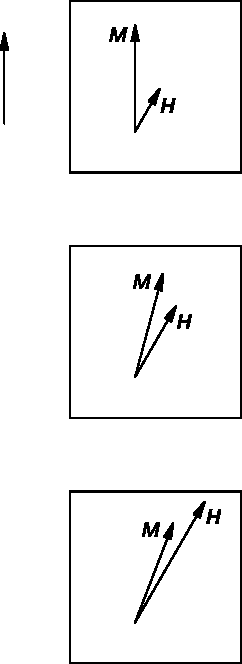
\includegraphics[width=0.7\linewidth]{fyz_fig0821.pdf}
      \caption{
               (\cite[s.~707]{Feynman02})}
      \label{fyz:fig0821}
    \end{figure}

    \begin{figure}[ht!] %\ref{fyz:fig0822}
      \centering
      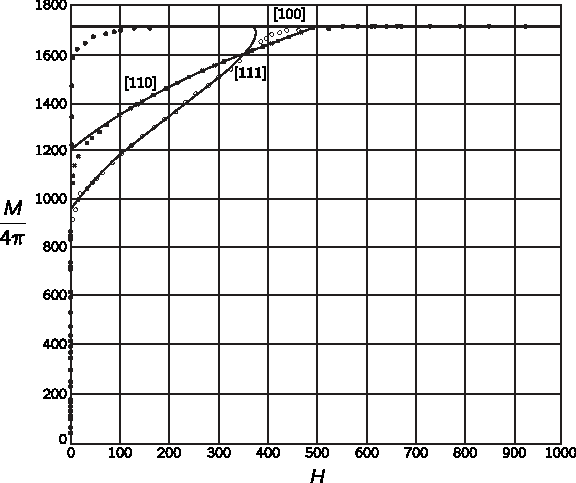
\includegraphics[width=0.7\linewidth]{fyz_fig0822.pdf}
      \caption{
               (\cite[s.~707]{Feynman02})}
      \label{fyz:fig0822}
    \end{figure}

    \begin{figure}[ht!]
      \centering
      \subcaptionbox{\label{fyz:fig0823a}}{\luafigure[0.9]{fyz_fig0823a.pdf}}               \\
      \subcaptionbox{\label{fyz:fig0823b}}{\luafigure[0.9]{fyz_fig0823b.pdf}}               \\
      \subcaptionbox{\label{fyz:fig0823c}}{\luafigure[0.9]{fyz_fig0823c.pdf}}
      \caption{
               (\cite[s.~748]{Feynman02})}
      \label{fyz:fig0823}
    \end{figure}

    \begin{figure}[ht!]
      \centering
      \subcaptionbox{\label{fyz:fig0824a}}{\luafigure[0.9]{fyz_fig0824a.pdf}}               \\
      \subcaptionbox{\label{fyz:fig0824b}}{\luafigure[0.9]{fyz_fig0824b.pdf}}               \\
      \subcaptionbox{\label{fyz:fig0824c}}{\luafigure[0.9]{fyz_fig0824c.pdf}}
      \caption{
               (\cite[s.~748]{Feynman02})}
      \label{fyz:fig0824}
    \end{figure}

    \begin{figure}[ht!] %\ref{fyz:fig0825}
      \centering
      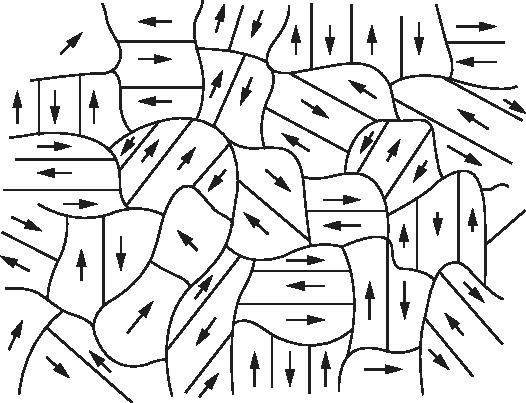
\includegraphics[width=0.7\linewidth]{fyz_fig0825.pdf}
      \caption{
               (\cite[s.~707]{Feynman02})}
      \label{fyz:fig0825}
    \end{figure}

    \begin{figure}[ht!] %\ref{fyz:fig0826}
      \centering
      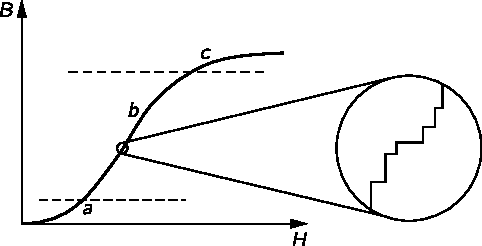
\includegraphics[width=0.7\linewidth]{fyz_fig0826.pdf}
      \caption{
               (\cite[s.~707]{Feynman02})}
      \label{fyz:fig0826}
    \end{figure}

    \begin{figure}[ht!] %\ref{fyz:fig0827}
      \centering
      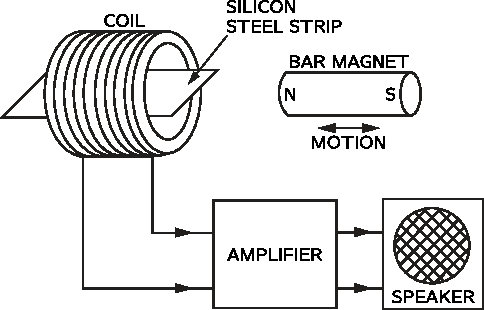
\includegraphics[width=0.7\linewidth]{fyz_fig0827.pdf}
      \caption{
               (\cite[s.~707]{Feynman02})}
      \label{fyz:fig0827}
    \end{figure}

    \begin{figure}[ht!] %\ref{fyz:fig0828}
      \centering
      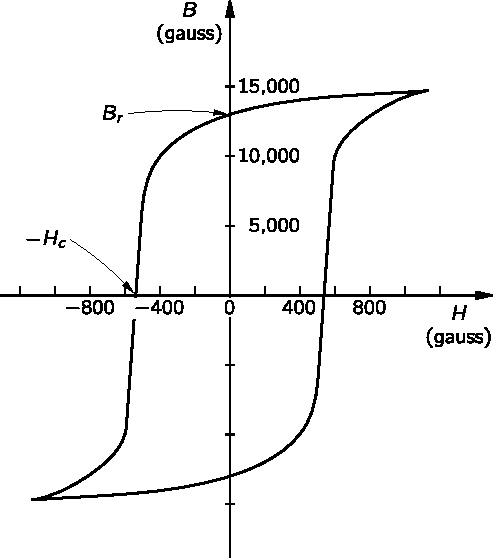
\includegraphics[width=0.7\linewidth]{fyz_fig0828.pdf}
      \caption{
               (\cite[s.~707]{Feynman02})}
      \label{fyz:fig0828}
    \end{figure}

    \begin{figure}[ht!] %\ref{fyz:fig0829}
      \centering
      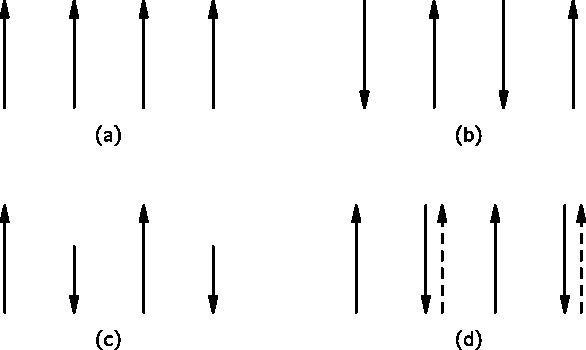
\includegraphics[width=0.7\linewidth]{fyz_fig0829.pdf}
      \caption{
               (\cite[s.~707]{Feynman02})}
      \label{fyz:fig0829}
    \end{figure}
s
    \begin{figure}[ht!] %\ref{fyz:fig0830}
      \centering
      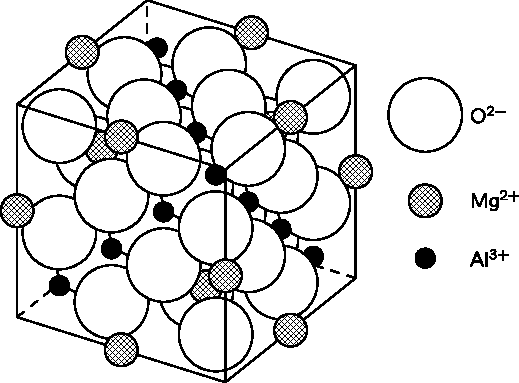
\includegraphics[width=0.7\linewidth]{fyz_fig0830.pdf}
      \caption{
               (\cite[s.~707]{Feynman02})}
      \label{fyz:fig0830}
    \end{figure}

    \todo[inline]{Kapitola fey2ch37 je nedodělaná, obsahuje pouze obrázky}

%} %tikzset
%---------------------------------------------------------------------------------------------------